In order to evaluate the performance of our system we examined the percentage of frames 
correctly classified with our segmentation and with perfect segmentation. The perfect
segmentation and ground truth label for each frame were determined using the annotation
to the development data.

The percentage of frames correct given perfect segmentation gives a sense of how well the
classification stage of our system performs. Currently, given perfect segmentation,
our system correctly classifies 63\% of frames. 

The percentage of frames correct with segmentation determined by our system when compared to the other metric
gives a good sense of how segmentation affects classification. With our segmentation, the 
system correctly classified 36\% of frames.

The confusion matricies of classifier stages of the perfectly segmented events, as well as the events segmented using our algorithm can be seen in Figure \ref{fig:confmat_perfect} and Figure \ref{fig:confmat_seg} respectively. (We need to make the figure bigger...)

\begin{figure}[h]
  \centering
  \centerline{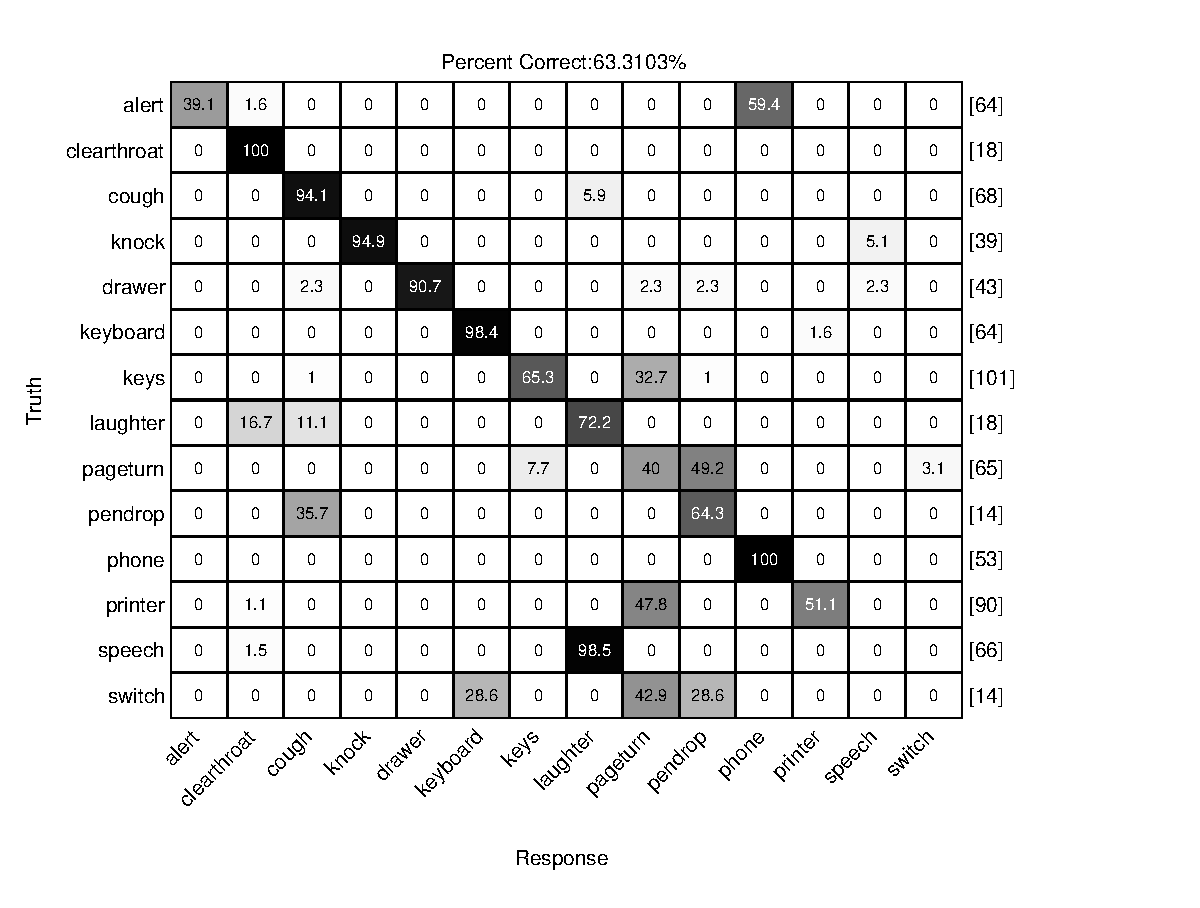
\includegraphics[width=\columnwidth]{confmatrix1}}
  \caption{Example of a figure with experimental results.}
  \label{fig:confmat_perfect}
\end{figure}

\begin{figure}[h]
  \centering
  \centerline{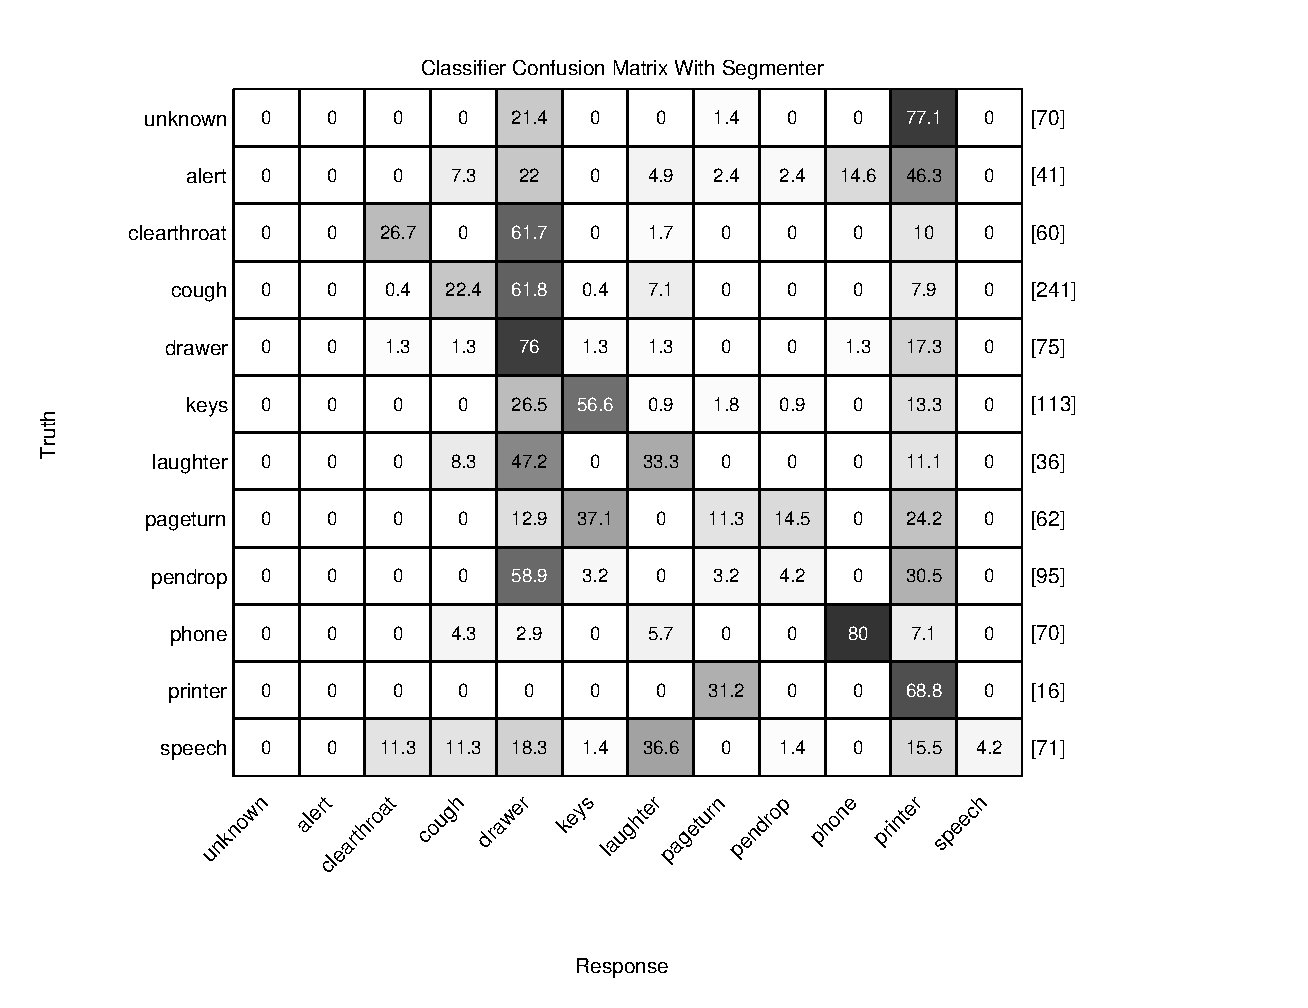
\includegraphics[width=\columnwidth]{confmatrix2}}
  \caption{Example of a figure with experimental results.}
  \label{fig:confmat_seg}
\end{figure}

It is worth noting that the above only hold for frame based classification. Our system was
not able to classify events as well as frames. The class of an event was chosen by taking 
the class chosen most often in the set of frames that formed the event. Because our system
is not able to accurately classify more than 50% of frames with our segmentation this method
of classifying events does not perform well.  